\documentclass[conference]{IEEEtran}
\IEEEoverridecommandlockouts
\usepackage[nocompress]{cite}
\usepackage{amsmath,amssymb,amsfonts}
\usepackage{graphicx}
\usepackage{textcomp}
\usepackage{booktabs}
\usepackage{url}

\begin{document}

\title{Seeing Through the Clouds: A Leakage-Controlled, Spatially Held-Out Test of Sentinel-1 Radar for Optical Vegetation Gaps in Burundi}

\author{
\IEEEauthorblockN{Kana Am\'ed\'ee}
\IEEEauthorblockA{Independent Researcher \\
Bujumbura, Burundi \\
kanaamedee00@gmail.com \\
ORCID 0009-0009-9620-6399 \\
Code: github.com/kanaamedee11/seeing-through-the-clouds-sar-gapfilling}
}

\maketitle

\par\noindent{\small\bfseries\itshape Abstract. }{\small\bfseries Cloud cover leaves gaps in optical vegetation time series, and radar is often proposed to fill them, but the gain over simple temporal methods is rarely measured with a test that mimics real use. We build a monthly Sentinel-2 NDVI and Sentinel-1 backscatter panel for 7{,}700 stratified points across Burundi (2019 to 2025, seven land-cover classes), hide real clear observations in gaps of 1, 3 and 6 months, and compare climatology, linear interpolation, gradient-boosted models with and without radar, and a radar-only model. Models are trained on 2019 to 2023 and tested on 2024 to 2025 at spatially held-out 0.25$^\circ$ blocks (five folds, 167{,}618 test targets per gap length), with confidence intervals from a pixel-cluster bootstrap. Radar helps modestly: it lowers RMSE by 2.2\% (95\% interval 2.0 to 2.5) for 1-month gaps, 3.4\% (3.1 to 3.8) for 3 months and 5.4\% (4.8 to 6.1) for 6 months relative to the same model without radar, and it beats interpolation by 10\% to 34\%. The gain varies strongly by land cover, from about zero in built-up land to 12\% in wetlands at 6 months. Radar alone, with no neighbouring optical value, cuts the RMSE of climatology by 14\%. In this data, however, natural gaps are short (86\% last one month, 2.4\% three or more), so the realistic gain is near 2\%. Finally, a single conformal prediction interval gives 90\% coverage overall but only 81\% in wetlands and 96\% in built-up land; class-conditional (Mondrian) calibration restores 90\% in every class. A check on an image tile excluded from training (Bujumbura and the Imbo plain, 100\,m, 23 target months) confirms that the learned models beat interpolation by 25\% and a simple blend by 4\%, but cannot confirm the radar gain on its own: it is 0.75\% (interval $-0.5$ to 2.0), consistent with the 1.7\% expected from the tile's land-cover mix. We state the limits: point samples without spatial context, NDVI only, two test years, and a class-stratified sample that does not estimate national totals.\par}
\vspace{0.6\baselineskip}
\par\noindent{\small\bfseries\itshape Keywords. }{\small\bfseries Gap filling, Sentinel-1, Sentinel-2, NDVI, SAR-optical fusion, conformal prediction, spatial cross-validation, Burundi\par}

\section{Introduction}

Vegetation indices such as NDVI from Sentinel-2 \cite{drusch2012s2} are the standard input for crop monitoring, drought warning and land-cover change. In the humid tropics, clouds make optical series incomplete, and Sentinel-1 radar \cite{torres2012s1}, which sees through cloud, is the usual proposed substitute. Methods that combine the two have been developed, including deep networks for cloud removal \cite{meraner2020cloud} and Gaussian processes for leaf-area gap filling \cite{pipia2019fusing}. What is harder to find is a plain answer to a practical question: how much better than interpolating between the clear months on either side does radar make the estimate, how does that depend on gap length and land cover, and how far can the stated uncertainty be trusted?

This paper answers that question for Burundi, a small, hilly, cloudy country, using free data in Google Earth Engine \cite{gorelick2017gee}. We take care with three issues that often make fusion results look better than they are. First, test pixels are in spatial blocks never seen in training, and test years are never seen in training, since nearby pixels and neighbouring months are strongly correlated \cite{roberts2017cv}. Second, the baselines include the obvious temporal ones, not only a weak straw man. Third, uncertainty is reported with conformal intervals \cite{lei2018distribution} and checked class by class.

The contributions are:
\begin{enumerate}
\item \textbf{A leakage-controlled gap-filling benchmark} for Burundi with real held-out clear observations as ground truth (Section~\ref{sec:method}).
\item \textbf{A measured value of radar} as a function of gap length and land cover, with intervals (Section~\ref{sec:results}).
\item \textbf{A calibration check} showing that one global conformal interval is mis-calibrated by class, and that class-conditional calibration fixes it (Section~\ref{sec:conf}).
\item \textbf{A reproducible pipeline:} one Earth Engine script and the analysis code reproduce every number and figure.
\end{enumerate}

\section{Data and Methods}
\label{sec:method}

\subsection{Sample and monthly panel}
We sample 1{,}100 points in each of seven ESA WorldCover 2021 classes \cite{zanaga2022wc} (tree, shrub, grass, crop, built-up, bare, wetland) inside Burundi, 7{,}700 points in all, so that rare classes are not drowned out. For each month from January 2019 to December 2025 (84 months) we export:
\begin{itemize}
\item the median Sentinel-2 surface-reflectance NDVI of clear observations (cloud, shadow and snow removed with the scene classification; granules with more than 70\% cloud skipped), and the number of clear observations;
\item the monthly mean Sentinel-1 VV and VH backscatter in dB (IW mode, both orbits);
\item the monthly CHIRPS rainfall total \cite{funk2015chirps};
\item elevation and slope from SRTM \cite{farr2007srtm}, latitude and longitude.
\end{itemize}
Missing optical values are kept as missing. Radar is almost always available (every pixel-month in the table). Sentinel-1B stopped acquiring in December 2021 \cite{esa2022s1b}, so radar sampling is denser in 2019 to 2021 than later. Radar values are clipped to physical ranges (VV from $-30$ to $5$\,dB, VH from $-35$ to $0$\,dB).

\subsection{Gap simulation}
For a target (point, month) with an observed NDVI value, we hide a window of $L$ consecutive months that contains the target, at a random position, with $L\in\{1,3,6\}$. The optical context available to a method is only what lies outside the window: the nearest observed NDVI before the window and after it, and the time distance to each. The hidden window's values, including the target, are never used. Radar and rainfall stay available throughout, as they would in practice.

\subsection{Climatology without leakage}
The climatology for a point and calendar month is the mean of its observed NDVI in the training years (2019 to 2023). For training rows it is computed leaving out the row's own year, so that models cannot learn to copy a target that is part of its own predictor. For test years 2024 and 2025 it is the full training-year mean. Anomalies of the context values (observed minus climatology) are also provided as predictors.

\subsection{Methods compared}
\begin{itemize}
\item \textbf{B0, climatology.} \textbf{B1, linear interpolation} in time between the two context values (the nearest one if only one exists). \textbf{B2, blend:} linear regression of the target on interpolation and climatology.
\item \textbf{M1, optical only:} histogram gradient boosting \cite{friedman2001gbm,pedregosa2011sklearn} on climatology, interpolation, context values, their time distances and anomalies, rainfall (this month and two previous), calendar month (sine and cosine), elevation, slope, coordinates and land-cover class.
\item \textbf{M2, optical + SAR:} M1 plus VV, VH, VV$-$VH, and VV and VH of the previous and next months.
\item \textbf{M3, SAR + climatology:} no neighbouring optical values at all; only climatology, radar, rainfall and static layers.
\end{itemize}
M1 and M2 differ only in the radar predictors, so their difference isolates what radar adds. Hyperparameters are fixed (250 iterations, learning rate 0.08, 31 leaves) and were not tuned on the test data. Each model is trained on at most 250{,}000 random training rows.

\subsection{Evaluation}
Points are grouped into 52 spatial blocks of $0.25^\circ\times0.25^\circ$ and assigned to five folds. For each fold, models are trained on the other four folds in 2019 to 2023 and tested on the held-out fold in 2024 and 2025. Results pool the five folds (167{,}618 test targets per gap length). The error measure is RMSE of NDVI; MAE and $R^2$ are also computed. Intervals on RMSE differences come from a bootstrap that resamples points (pixel clusters), since all months of a point are correlated (1{,}000 draws, 400 for class-level results).

\subsection{Calibrated intervals}
For the best model we form 90\% prediction intervals by split conformal prediction on absolute residuals \cite{lei2018distribution}. The calibration residuals for a test fold are those of the other four folds in the test years, which is a cross-conformal scheme in the spirit of the jackknife+ \cite{barber2021jackknifeplus}. We compare a global quantile with class-conditional (Mondrian) quantiles \cite{vovk2012conditional}.

\section{Results}
\label{sec:results}

\subsection{How long are real gaps?}
Across all 7{,}700 points, 9.6\% of monthly NDVI values are missing. Of the 52{,}861 natural gaps, 85.8\% last one month, 11.7\% two months, 2.4\% three months or more, and 0.05\% six or more (maximum 7). Missing values concentrate in the rainy months: 25.9\% of values are missing in November and 19.5\% in April, against under 1\% in July and August (Fig.~\ref{fig:gaps}). This matters for interpretation: our 3- and 6-month tests describe what would happen in cloudier places or with stricter quality filters, not typical Burundian gaps.

\begin{figure}[t]
\centering
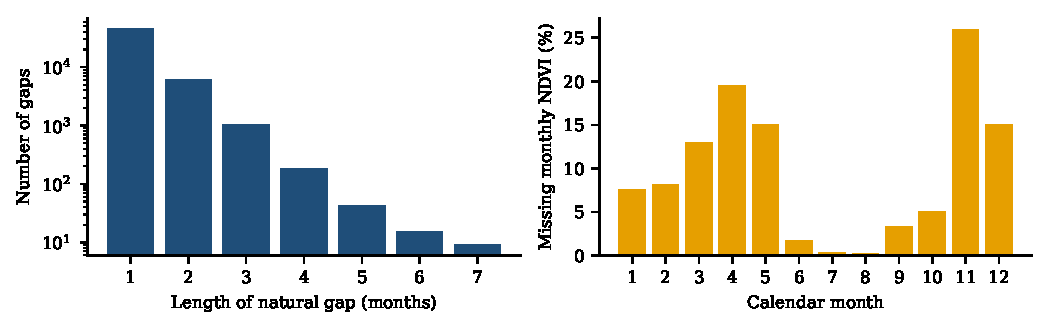
\includegraphics[width=\columnwidth]{figures/fig_gaps.pdf}
\caption{Natural gaps in the monthly Sentinel-2 NDVI panel. Left: gap lengths (log scale). Right: share of missing values by calendar month.}
\label{fig:gaps}
\end{figure}

\subsection{Accuracy by method and gap length}
\begin{table}[t]
\centering
\caption{RMSE of NDVI on held-out blocks and years (2024 to 2025), by gap length. Lower is better. Climatology and M3 do not use neighbouring optical values, so they do not depend on $L$ (small differences for M3 at $L=1$ come from a different random draw).}
\label{tab:rmse}
\begin{tabular}{lccc}
\toprule
Method & 1 month & 3 months & 6 months \\
\midrule
B0 climatology & 0.136 & 0.136 & 0.136 \\
B1 linear interpolation & 0.102 & 0.133 & 0.156 \\
B2 blend & 0.098 & 0.114 & 0.122 \\
M1 ML, optical only & 0.094 & 0.102 & 0.108 \\
M2 ML, optical + SAR & \textbf{0.092} & \textbf{0.099} & \textbf{0.102} \\
M3 ML, SAR + climatology & 0.116 & 0.116 & 0.116 \\
\midrule
$R^2$ of M2 & 0.841 & 0.814 & 0.801 \\
\bottomrule
\end{tabular}
\end{table}
Linear interpolation is competitive at one month but becomes worse than climatology at three months and clearly worse at six (Table~\ref{tab:rmse}, Fig.~\ref{fig:rmse}). Learning to combine interpolation, climatology and rainfall (M1) removes most of that loss. Adding radar (M2) lowers RMSE further at every gap length.

\begin{figure}[t]
\centering
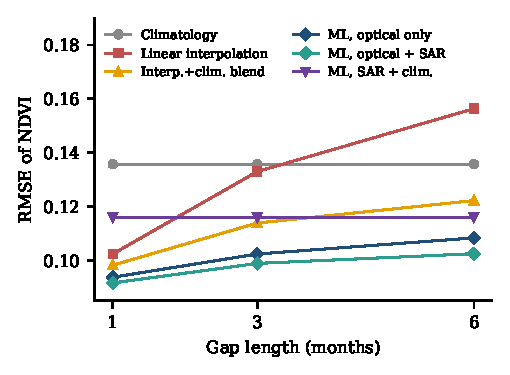
\includegraphics[width=\columnwidth]{figures/fig_rmse.pdf}
\caption{RMSE of NDVI against gap length for the six methods.}
\label{fig:rmse}
\end{figure}

\subsection{What radar adds}
Relative to the same model without radar (M2 against M1), RMSE falls by 2.2\% at one month (95\% interval 2.0 to 2.5), 3.4\% at three months (3.1 to 3.8) and 5.4\% at six months (4.8 to 6.1). Relative to linear interpolation, M2 is 10.5\% (10.0 to 11.0), 25.6\% (25.1 to 26.3) and 34.5\% (33.9 to 35.0) better, but most of that (80\% to 90\%) comes from the machine-learning combination and not from radar: M1 alone is 8.4\%, 23.0\% and 30.7\% better than interpolation. Against the simple blend B2, M2 is 6.7\%, 13.2\% and 16.1\% better. All intervals exclude zero. The radar gain therefore grows with gap length, as expected, since the less optical information remains the more a second sensor matters.

Radar by itself carries real information about vegetation: M3, with no neighbouring optical value at all, reduces RMSE by 14.5\% (12.3 to 16.5) relative to climatology. But it does not approach models that have a clear neighbouring month (RMSE 0.116 against 0.092 to 0.102).

\subsection{Where radar helps}
\begin{figure}[t]
\centering
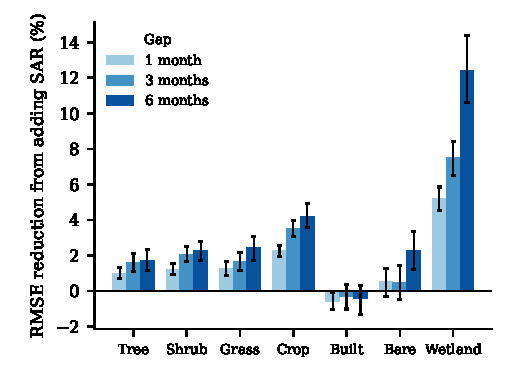
\includegraphics[width=\columnwidth]{figures/fig_gain.pdf}
\caption{RMSE reduction from adding SAR (M2 against M1) by land-cover class and gap length, with 95\% pixel-cluster bootstrap intervals.}
\label{fig:gain}
\end{figure}
The gain is far from uniform (Fig.~\ref{fig:gain}). It is largest in wetlands (5.2\%, 7.5\% and 12.4\% at 1, 3 and 6 months), where backscatter responds strongly to flooding and to emergent vegetation that NDVI alone may not track. It is moderate in cropland (2.3\%, 3.5\%, 4.2\%), shrub and grass (1.2\% to 2.5\%) and trees (1.0\% to 1.7\%). In built-up land radar does not help (about $-0.6\%$ at one month, with an interval from $-1.0$ to $-0.1$, and indistinguishable from zero at 3 and 6 months), and in bare land only at 6 months (2.3\%, interval 1.2 to 3.4). Averaged over classes the gain is therefore driven mainly by wetlands and crops. By calendar month the 6-month gain varies between 4.1\% (April) and 8.7\% (July), with no sharp seasonal pattern.

\subsection{Uncertainty}
\label{sec:conf}
\begin{figure}[t]
\centering
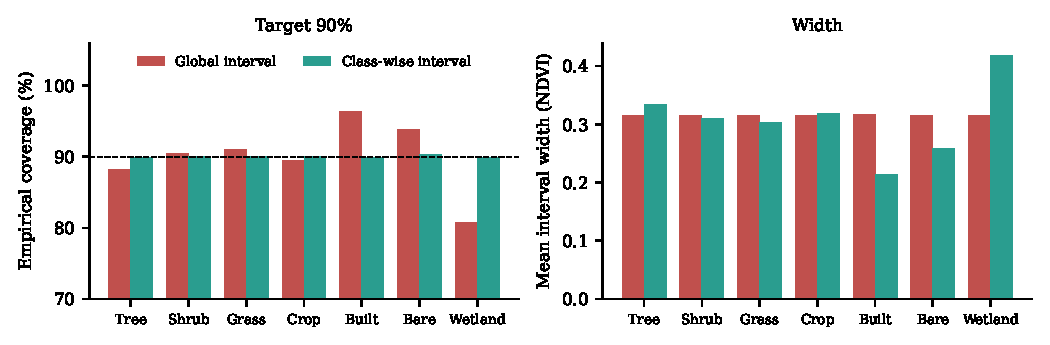
\includegraphics[width=\columnwidth]{figures/fig_conf.pdf}
\caption{90\% conformal intervals for M2 at a 3-month gap, by class. A single global interval is too wide for built-up and bare land and too narrow for wetland and trees; class-conditional calibration corrects coverage.}
\label{fig:conf}
\end{figure}
A single global interval has the right coverage overall (90.0\% at every gap length) but not within classes (Fig.~\ref{fig:conf}, 3-month gap): coverage is 80.7\% in wetlands, 88.2\% in trees, 96.4\% in built-up land and 93.9\% in bare land. This is the usual failure of marginal guarantees: errors are much larger in some classes than others, so a pooled quantile over-covers the easy classes and under-covers the hard one. Class-conditional (Mondrian) calibration brings coverage to 89.9\% to 90.3\% in every class. Mean width changes from 0.315 for all classes to 0.214 in built-up land and 0.258 in bare land, but widens to 0.418 in wetlands. The overall mean width is almost unchanged (0.308 against 0.315), so the correction costs nothing on average and gives users honest, class-specific intervals.

\subsection{Check on an unseen image tile}
\label{sec:tile}
The point experiment never shows the method on an image, and its test blocks, though held out, are samples. We therefore ran a second check on a 100\,m monthly tile of Bujumbura and the Imbo plain (24.7 by 26.7\,km, 267 by 247 pixels, same variables). The models were retrained on the point panel using only points more than $0.1^\circ$ outside the tile, 3-month gaps and years 2019 to 2023, and then applied to every land pixel of the tile. For each target month from January 2024 to November 2025 (23 months) a 3-month window centred on the target was hidden, as before. Rainfall is the tile mean. Water is excluded.

\begin{figure*}[t]
\centering
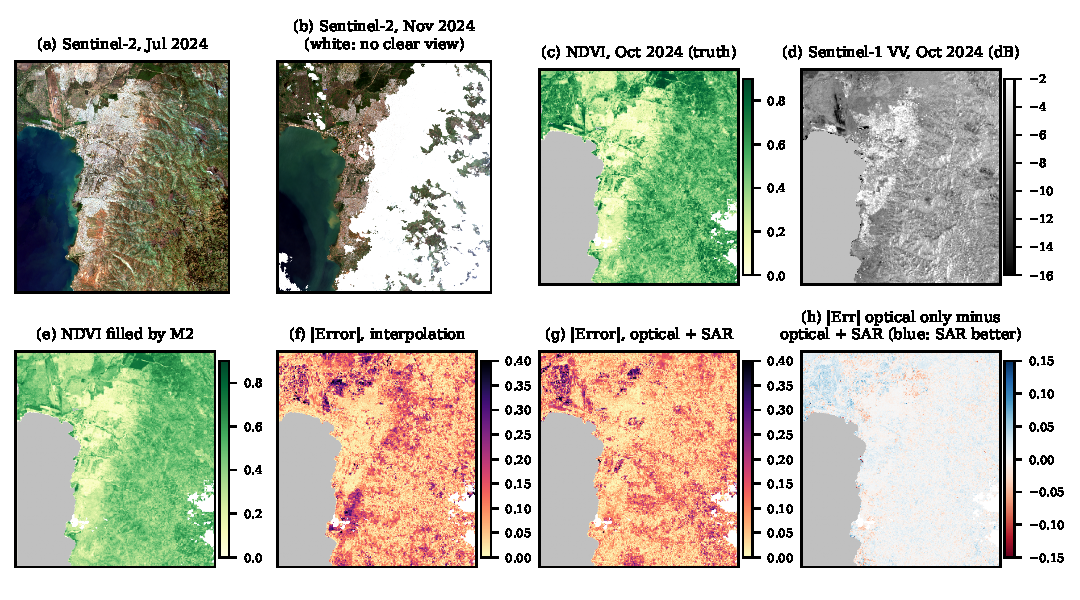
\includegraphics[width=\textwidth]{figures/fig_tile.pdf}
\caption{Image-tile check, target month October 2024 with September to November hidden. Top: clear-view Sentinel-2 true colour in July and November 2024, observed NDVI in October (the truth) and Sentinel-1 VV. Bottom: NDVI filled by the optical + SAR model, absolute errors of linear interpolation and of the optical + SAR model, and the difference in absolute error between the optical-only and optical + SAR models (blue where radar helps).}
\label{fig:tile}
\end{figure*}
Figure~\ref{fig:tile} shows the target month. November 2024 is a real cloud gap: only 53\% of pixels have a clear NDVI value that month. Filling October by the optical + SAR model gives an RMSE of 0.096, against 0.108 for linear interpolation, 0.100 for the optical-only model and 0.090 for the simple blend; radar helps in 58\% of pixels, but the difference between the two models is small and spatially mixed (Fig.~\ref{fig:tile}h). Across all 23 months, mean RMSE is 0.134 (interpolation), 0.105 (blend), 0.101 (optical only) and 0.1008 (optical + SAR). The optical + SAR model beats interpolation in 21 of 23 months (24.9\% lower mean RMSE) and the blend in 17, and the optical-only model is 4.1\% better than the blend, so these orderings from the point test are reproduced. The radar gain itself is not: the mean monthly reduction relative to the optical-only model is 0.75\% (95\% interval over months $-0.5$ to 2.0), and the radar model is better in only 12 of 23 months. Pooled over months, the gain is near zero in trees (about $-0.1\%$), shrub (0.1\%), grass (0.2\%) and crops ($-0.5\%$) and negative in built-up land ($-2.3\%$) and in the 188 wetland pixels ($-3.5\%$). Weighting the point-test class gains at 3 months by this tile's land-cover mix predicts a gain of 1.7\%, which lies inside the tile's interval. The tile is therefore consistent with a small radar gain but does not demonstrate it; it cannot, by itself, separate a 2\% gain from none. We did not isolate why the wetland gain of the point test does not appear here, where wetlands are rare, nor the effect of the coarser 100\,m sampling of radar and optical data.

\section{Discussion and Limitations}

For a user in Burundi the practical answer is mixed. In the point test radar gives a real but small improvement at the gap lengths that actually occur (about 2\% at one to two months), a larger one if gaps are long, and most in wetlands and cropland; the image-tile check did not reproduce this on its own, so we regard the radar gain as small and class-dependent, and the larger and more certain gains as those from combining temporal context with climatology and rainfall. Most of the benefit over interpolation comes from using climatology and rainfall to correct it. If a project only has radar and no recent clear optical image, radar alone still cuts the RMSE of climatology by 14\% (against 25\% to 33\% for the best model), which can be enough for coarse monitoring.

Limits of this study:
\begin{enumerate}
\item The sample is stratified by class with equal numbers, so pooled RMSE is not an estimate for Burundi as a whole; class-level results are the meaningful ones.
\item Models see single 20\,m pixels and no spatial neighbourhood. A convolutional network on image patches may use radar texture better; we have not tested that.
\item The target is NDVI only, from monthly medians. Residual undetected cloud or haze in the optical ``truth'' adds noise to the target and so inflates the RMSE of all methods.
\item Only two test years, both after the end of Sentinel-1B. Training years 2019 to 2021 have denser radar sampling, so there is a change in radar noise between training and test. This may reduce or increase the radar gain; we did not separate it.
\item Radar features use the next month as well as the previous one, which is fine for retrospective gap filling but not for real-time use.
\item Hyperparameters were fixed, not tuned; a tuned model might differ in detail, and since all gradient-boosted models share settings we expect, but have not shown, that the ordering of methods would hold.
\item The image-tile check covers one area at 100\,m, with few wetland pixels, and 23 correlated months; it neither confirms nor refutes a radar gain of about 2\%.
\item Conformal coverage is checked on exchangeable blocks within test years; under a different year or region, coverage can drift.
\end{enumerate}

\section{Conclusion}

Under a test that holds out both places and years, adding Sentinel-1 radar lowers the error of Sentinel-2 NDVI gap-filling in Burundi by 2\% to 5\% on top of a model that already uses climatology, rainfall and the surrounding clear months, and by up to 34\% relative to linear interpolation. The gain grows with gap length and is concentrated in wetlands and crops. Real gaps in this data are short, so the realistic benefit is near the low end, and a check on an unseen image tile was consistent with, but too noisy to confirm, a gain of that size. A single conformal interval hides large differences in coverage between land-cover classes (81\% to 96\% against a 90\% target); class-conditional calibration removes them at no cost in average width.

\bibliographystyle{IEEEtran}
\bibliography{references}

\end{document}
